\documentclass[12pt,a4paper]{report}
\usepackage[margin=3cm]{geometry}
\usepackage{ngerman}
\usepackage[utf8]{inputenc}
\usepackage[onehalfspacing]{setspace}
\usepackage[numbers,round]{natbib}
\usepackage{graphicx}
\usepackage[colorlinks,
pdfpagelabels,
pdfstartview = FitH,
bookmarksopen = true,
bookmarksnumbered = true,
linkcolor = black,
plainpages = false,
hypertexnames = false,
citecolor = black] {hyperref}

\begin{document}


\pagenumbering{roman}
\thispagestyle{empty}
\begin{verbatim}





\end{verbatim}
\begin{center}
\textbf{\huge{Semantische Beziehungen in Texten mit Word2Vec }}\\
\begin{verbatim}
\end{verbatim}
\textbf{\large{und der Vergleich zwischen allgemeinen und domänenspezifischen Korpora als Trainingsdaten}}
\end{center}
\begin{verbatim}



\end{verbatim}
\begin{center}
\large B A C H E L O R A R B E I T

\begin{verbatim}
\end{verbatim}

\end{center}
\begin{center}
im Studiengang\\
\textsc{Medieninformatik (MI7)}\\
an der Hochschule der Medien in Stuttgart\\
vorgelegt von \textsc{Ruben Müller}\\
\begin{verbatim}
\end{verbatim}
im Juli 2015


\end{center}
\begin{verbatim}







\end{verbatim}

\begin{flushleft}
\begin{tabular}{lll}
\textbf{Erstprüfer:} & & \textsc{Prof. Dr-Ing. Johannes Maucher},\\ 
&&\small Hochschule der Medien, Stuttgart  \\
\textbf{Zweitprüfer:} & & \textsc{M.Sc. Andreas Stiegler},\\
&&\small Hochschule der Medien, Stuttgart\\
\end{tabular}
\end{flushleft}

\newpage
\chapter*{Erklärung}
Hiermit versichere ich, Ruben Müller, an Eides Statt, dass ich die vorliegende
Bachelorarbeit mit dem Titel: \glqq Semantische Beziehungen in Texten mit Word2Vec\grqq{} selbständig und ohne fremde Hilfe verfasst und keine anderen als die angegebenen
Hilfsmittel benutzt habe. Die Stellen der Arbeit, die dem Wortlaut oder dem Sinn nach anderen
Werken entnommen wurden, sind in jedem Fall unter Angabe der Quelle kenntlich gemacht. Die
Arbeit ist noch nicht veröffentlicht oder in anderer Form als Prüfungsleistung vorgelegt worden.\\
Ich habe die Bedeutung der eidesstattlichen Versicherung und die prüfungsrechtlichen Folgen (§ 23 Abs. 2 Bachelor-SPO (7 Semester) der HdM) sowie die strafrechtlichen Folgen (gem. § 156 StGB) einer unrichtigen oder
unvollständigen eidesstattlichen Versicherung zur Kenntnis genommen.\\
\vspace{1em}\\
Filderstadt, den XX. Juli 2015\\
\vspace{5em}\\
Ruben Müller


\newpage
\chapter*{Kurzfassung}
Diese Bachelorthesis beschäftigt sich mit der Analyse von semantischen Beziehungen innerhalb mit Word2Vec gelernten Modellen.
\\Dazu sollen zum einen schon der vorhandene allgemeine Wikipedia-Korpus gelernt und analysiert werden, was als semantisch ähnlich erkannt wird. Zum anderen soll ein Korpus über eine spezielle Domäne erstellt und gelernt werden. Welche spezielle Domäne analysiert und verglichen werden soll, wird im Laufe der Bearbeitung festgelegt.
\\Diese beiden Korpora sollen sich dann gegenüber gestellt und analysiert werden, was jeweils als semantisch ähnlich erkannt wird. 
\\Ziel dieser Arbeit soll es sein, festzustellen ob ein allgemeiner Korpus oder ein spezieller Domänenkorpus genauere Resultate im Hinblick auf semantische Ähnlichkeiten erzielt. Anstatt eines allgemeinen Korpus zu verwenden, könnte es sich dann anbieten zwischen mehreren speziellen Korpora auszuwählen, je nachdem welche Domäne aktuell bearbeitet werden soll.
\newpage
\chapter*{Abstract}
\newpage
\tableofcontents
\newpage
\chapter*{Begriffsverzeichnis}
	\begin{tabular}{r|l}	
	\textbf{Begriff} & Erklärung\\
	\hline	
	\textbf{Ähnliche Worte} & Im Word2Vec-Modell, mit der Methode\\
	& \textit{most\_similar()}, erhaltene Worte.\\
	\textbf{SVM} & Support Vector Machine\\
	\textbf{NBC} & Naive Bayes Classifier\\
	\textbf{CBOW} & Continuous bag-of-words\\

\end{tabular}
\newpage
\pagenumbering{arabic}
\chapter{Einleitung}
	\section{Motivation}
	
	\section{Problemstellung}
	\section{Aufbau der Arbeit}

\newpage
\chapter{Daten und Vorverarbeitung}
	\section{Datenbasis}
	Zum erfolgreichen Training des Word2Vec Modells wird eine sehr große Menge an Daten gebraucht\footnote{In \cite{DBLP:journals/corr/MikolovSCCD13} werden Trainingsdaten mit bis zu 30 Milliarden Wörtern benutzt.}. 
	Für den ersten Korpus wurde der komplette englischsprachige Wikipedia Korpus verwendet\footnote{Dump von März 2015, http://dumps.wikimedia.org/enwiki/latest/enwiki-latest-pages-articles.xml.bz2, abgerufen am 09.04.2015}. Dieser enthält 8.392.453 Artikel, 242.144.317 Sätze und 2.919.802.692 Worte.\\
	Der zweite in der Arbeit verwendete Korpus besteht auch aus Wikipedia Artikeln, allerdings wurden hier nur technologiespezifische Artikel verwendet. Der komplette englische Wikipedia Korpus wurde zuerst in die einzelnen Artikel aufgeteilt und diese wurden dann mit einem NBC in die Klassen \textit{tech, entertainment, sport, science, politic} eingeteilt.\\
	


	\section{Externe Programme und Hilfsmittel}
	Dieser Abschnitt enthält eine Auflistung mit kurzen Beschreibungen, der in dieser Arbeit verwendeten Hilfsmittel und externen Programme.\\
	\vspace{1em}\\	
	\textbf{gensim}\cite{rehurek_lrec}\footnote{https://radimrehurek.com/gensim/, abgerufen am 24.06.2015} ist eine Bibliothek für Python. Sie enthält unter anderem eine performanzoptimierte Implementierung von Word2Vec.\\ 
	\vspace{1em}\\
	Der \textbf{NBC}, der zum Klassifizieren der Artikel verwendet wurde, ist der im DataMining Praktikum selbst implementierte.
	\vspace{1em}\\
	
	\section{Vorverarbeitung}
	\label{sec:Vorverarbeitung}
	Der komplette Wikipediadump kann als komprimierte XML-Datei heruntergeladen werden\footnote{http://dumps.wikimedia.org/enwiki/latest/enwiki-latest-pages-articles.xml.bz2, abgerufen am 09.04.2015} die entpackte XML-Datei hat eine Größe von 48,8 GB. Die Daten müssen zunächst bereinigt werden um als Trainingsdaten für Word2Vec Modelle zu dienen.\\		
	Um das Wiki-Markup, wie unter anderem Links, Referenzen oder Zitate, und die XML-Tags zu entfernen, kann ein schon vorgefertigtes Perl Skript von Matt Mahoney benutzt werden\footnote{http://mattmahoney.net/dc/textdata.html unter Appendix A, abgerufen am 25.06.2015}, welches von Mikolov et al. auf der Google Code Seite von Word2Vec vorgeschlagen wird\footnote{https://code.google.com/p/word2vec/, abgerufen am 25.06.2015}. Dieses Skript wurde speziell zum Bereinigen von Wikipediadaten erstellt und wurde leicht verändert, sodass Zahlen, Satzzeichen und die Groß- und Kleinschreibung erhalten bleibt. Außerdem werden die Umlaute in $ae$, $oe$ und $ue$ umgewandelt. Da die bis hierher bereinigten Daten eine Gesamtgröße von 18 GB haben, ist es nötig die Daten weiter aufzubereiten, sodass sie als Input für die Klasse $gensim.models.word2vec.LineSentence$\footnote{Diese Klasse kann auch als Input zum Trainieren des Word2Vec Modells genutzt werden.}, aus der Gensim Bibliothek dienen. Dazu müssen die einzelnen Sätze in je einer Zeile stehen, alle Worte klein geschrieben sein, frei von Satzzeichen und mit Leerzeichen getrennt sein.\\
	
	Um den kompletten Wikipediadump in die einzelnen Wikipedia Artikel aufzuteilen muss die XML-Datei mittels eines SAX-Parsers\footnote{xml.sax.handler.ContentHandler} geparst und dann in einzelne Dateien geschrieben werden. Diese einzelnen Dateien können dann mit dem Perl Skript gereinigt und dann mittels NBC klassifiziert werden. Nach der Klassifizierung können die Dateien wieder in eine große Datei zusammengefasst und weiter verarbeitet werden. Auch diese Daten müssen, wie der Gesamtkorpus, mit der Klasse $gensim.models.word2vec.LineSentence$ verarbeitet werden.
\newpage
\chapter{Word2Vec}
Im folgenden Kapitel wird kurz erklärt was Word2Vec\footnote{https://code.google.com/p/word2vec/} ist und welche wichtigen Parameter und Algorithmen bei der Berechnung von Word2Vec benutzt werden können.\\

In Word2Vec Modellen werden Worte als Vektoren dargestellt\footnote{Word2Vec heißt wörtlich Wort zu Vektor.}. Hier wird mittels \textit{distributed representation}\cite{DBLP:journals/corr/abs-1301-3781} ein n-dimensionaler Vektorraum erzeugt, in dem jedes Wort aus den Trainingsdaten durch einen Vektor dargestellt wird.\\
Als nächster Schritt werden die Vektoren in ein neuronales Netz gegeben und dort mittels eines Lernalgorithmus so verändert, dass Worte mit ähnlicher Bedeutung ähnliche Vektoren haben. So kann die Ähnlichkeit zwischen zwei Vektoren mit der Kosinus-Ähnlichkeit berechnet werden.\\
Die Berechnung der Wortvektoren kann mit neuronalen Netzen unterschiedlicher Architektur erreicht werden, \textit{CBOW} oder \textit{Skip-gram}. Desweiteren stehen unterschiedliche Lernalgorithmen für die neuronalen Netze zur Verfügung, \textit{hierarchical softmax}  und \textit{negative sampling}.\\
Beim Training können unterschiedliche Parameter eingestellt werden.\\



\begin{figure}[h]
  \begin{center}
	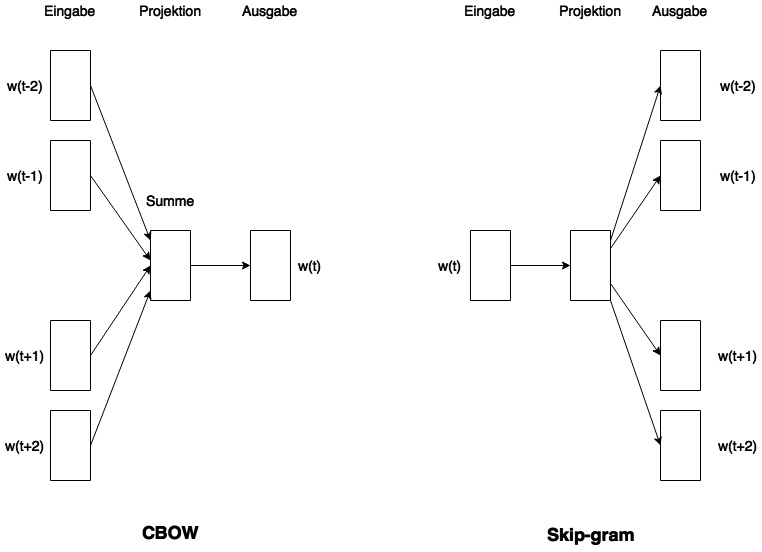
\includegraphics[scale=0.55]{CBOWvsSkip-gram.png}
  \end{center}  
  \caption{CBOW und Skip-gram im Vergleich, übersetzt nach \cite{DBLP:journals/corr/abs-1301-3781}}
  \label{cbowvsskipgram}
\end{figure}

	\section{Parameter}
	
	\textbf{size}
	\vspace{1em}\\
	Mit dem Parameter \textit{size} wird die Anzahl der Dimensionen der Wortvektoren eingestellt. In einem n-Dimensionalen Vektorraum nimmt n den Wert von \textit{size} an.\\	
	\vspace{1em}\\
	\textbf{window}
	\vspace{1em}\\
	\textit{window} ist der maximale Abstand innerhalb eines Satzes zwischen benachbarten Worten, die zur Berechnung der Wordvektoren betrachtet werden.\\
	\vspace{1em}\\
	\textbf{min\_count}
	\vspace{1em}\\
	Der Parameter \textit{min\_count} gibt an, wie oft ein Wort in den Testdaten mindestens vorkommen muss, um in das Wörterbuch aufgenommen zu werden.\\
	\vspace{1em}\\
	\textbf{negative}
	\vspace{1em}\\
	Dieser Parameter wird nur benötigt, wenn als Lernalgorithmus negative sampling verwendet wird.\footnote{siehe \ref{sec:negativeSampling} Negative sampling}
	
	\section{CBOW}
	CBOW ist die Abkürzung für Continuous bag-of-words (dt. stetige Menge an Worten). Beim CBOW wird ein neuronales Netz ohne verdeckte Schichten (hidden layer) verwendet\cite{DBLP:journals/corr/abs-1301-3781}.\\
	Im CBOW Model wird aus dem Kontext ein Wort vorhergesagt (siehe Abbildung \ref{cbowvsskipgram}). Die Anzahl, der aus dem Kontext zu verwendende Worte, wird mit dem Parameter \textit{window} angegeben.
	
	\section{Skip-gram}
	Beim Skip-gram Model wird auch wie beim CBOW Model ein neuronales Netz ohne verdeckte Schichten (hidden layer) verwendet \citep{DBLP:journals/corr/abs-1301-3781}.\\
	Allerdings wird hier nicht ein Wort aus dem Kontext vorhergesagt, sondern aus einem Wort wird der Kontext vorhergesagt (siehe Abbildung \ref{cbowvsskipgram}).\\
	
	Mehrere verdeckte Schichten in neuronalen Netzen machen die Modelle genauer, allerdings kommt auch die meiste Komplexität des ganzen Models von solchen verdeckten Schichten \citep{DBLP:journals/corr/abs-1301-3781}. Mikolov et al. haben deshalb neuronale Netze ohne verdeckte Schichten bevorzugt, da damit sehr große Datenmengen viel effizienter gelernt werden konnten.
	
	\section{Hierarchical softmax}
	Eine Annäherung an das allgemeine softmax ist das hierarchical softmax \citep{DBLP:journals/corr/MikolovSCCD13}. Der Hauptvorteil ist, dass anstatt W Ausgabeknoten im neuronalen Netz nur ungefähr $log_2(W) $ Knoten ausgewertet werden müssen um die Wahrscheinlichkeiten zu errechnen. \\
	Bei diesem Lernalgorithmus wird das Wörterbuch als Huffman Binärbaum dargestellt. Dies hat den weiteren Vorteil, dass häufig genutzte Worte kurze Kodierungen haben, was sich auf das Trainingstempo positiv auswirkt.
	
	\section{Negative sampling}
	\label{sec:negativeSampling}
	Alternativ zum hierarchical softmax kann das negative sampling als Lernalgorithmus für das neuronale Netz verwendet werden \citep{DBLP:journals/corr/MikolovSCCD13}.\\
	Das negative sampling unterscheidet sich zum hierarchical softmax insofern, dass nicht die Ähnlichkeiten zu anderen Worten berechnet werden, sondern es wird davon ausgegangen, dass zufällig ausgewählte Worte mit einer hohen Wahrscheinlichkeit unähnlich sind. Wie viele solcher zufällig ausgewählter Worte benutzt werden sollen kann mit dem Parameter \textit{negative} angegeben werden.
	

	
	
\newpage
\chapter{Wikipedia-Korpus}
Im Folgenden Kapitel werden die in der Arbeit verwendeten Korpora erläutert und die im Word2Vec Modell benutzten Parameter begründet.\\
Des weiteren werden die benutzten Testdaten vorgestellt.
\iffalse
	Kompletter Wikikorpus: \\
	8392453 Artikel\\
	wordcount: 2919802692\\
	sentencecount: 242144317\\
	
	
	Techkorpus:\\
	187144 Artikel (2,2%)\\
	wordcount: 9866096 (0,34%)\\
	sentencecount: 3166065 (1,3%)\\
\fi
	\section{Gesamtkorpus}
	\label{sec:Gesamtkorpus}
	Da sich die Qualität  der Wortvektoren im Word2Vec Modell wesentlich mit der Menge an Trainingsdaten erhöht, werden möglichst große Textkorpora bevorzugt. Auf der Google Code Seite von Word2Vec\footnote{https://code.google.com/p/word2vec/, abgerufen am 29.06.2015}, werden für Forschungszwecke einige Beispiele für online verfügbare große Korpora genannt. Unter anderem auch der neueste Wikipedia Auszug\footnote{http://dumps.wikimedia.org/enwiki/latest/enwiki-latest-pages-articles.xml.bz2, abgerufen am 29.06.2015}.\\
	Da in dieser Arbeit ein allgemeiner und ein domänenspezifischer Korpus als Trainingsdaten für das Word2Vec Modell verglichen werden sollen, eignet sich der Wikipedia Korpus gut. \\
	Wie in \ref{sec:Vorverarbeitung} beschrieben, mussten die Daten erst einer Säuberung unterzogen werden um dann anschließend im Word2Vec Modell trainiert zu werden. Der bereinigte, komplette englischsprachige Wikipedia Korpus\footnote{Dump von März 2015, http://dumps.wikimedia.org/enwiki/latest/enwiki-latest-pages-articles.xml.bz2, abgerufen am 09.04.2015} enthält 8.392.453 Artikel, 242.144.317 Sätze und 2.919.802.692 Worte.\\

Used: Skip-gram, hierarchical softmax.\\

Um die optimalen Parameter für das Training des Modells herauszufinden wurde ein kleinerer Wikipedia Auszug\footnote{http://mattmahoney.net/dc/enwik9.zip, abgerufen am 30.06.2015, beinhaltet die ersten 1 Milliarde Zeichen des Gesamtkorpus} benutzt und mit den unterschiedlichen Parametern gelernt und evaluiert (siehe Tabelle \ref{tab:VergleichParameter}).\\
Die Word2Vec-Klasse in der Gensim-Implementierung beinhaltet eine Evaluationsfunktion\footnote{\textit{gensim.models.word2vec.Word2Vec.accuracy(FILENAME)}}, die die Accuracy des Models berechnet. Die Funktion erwartet einen Dateinamen, in der jede Zeile ein 4-Tupel ist und die einzelnen Abschnitte mit \glqq : SECTION NAME\grqq{} unterteilt sind. Auf der Google Code Seite ist eine solche Datei als Beispiel vorhanden\footnote{https://code.google.com/p/word2vec/source/browse/trunk/questions-words.txt, abgerufen am 29.06.2015}. In diesem Beispiel sind 14 Kategorien\footnote{\textit{capital-common-countries, capital-world, currency, city-in-state, family, gram1-adjective-to-adverb, gram2-opposite, gram3-comparative, gram4-superlative, gram5-present-participle, gram6-nationality-adjective, gram7-past-tense, gram8-plural, gram9-plural-verbs}} mit insgesamt 19544 4-Tupel aufgelistet.\\

\begin{table}[h]
\caption{Vergleich Parameter}
\begin{center}
\begin{tabular}{l|l|l|l}\\
\textbf{Size} & \textbf{Window\footnote{Auf der Google Code Seite von Word2Vec (https://code.google.com/p/word2vec/, abgerufen am 29.05.2015) wird eine window size beim Skip-gram Modell von um die 10 vorgeschlagen.}} & \textbf{Min\_count} & \textbf{Gesamtaccuracy}\\
\hline	
400 & 10 &  5 & 52.9\%\\
400 & 10 & 10 & 52.5\%\\
300 & 10 &  5 & \textbf{53.3\%}\\
300 & 10 & 10 & 52.9\%\\
200 & 10 &  5 & 50.5\%\\
200 & 10 & 10 & 50.5\%\\
100 & 10 &  5 & 42.0\%\\
100 & 10 & 10 & 41.3\%\\

\end{tabular}
\end{center}
\end{table}

Auf dem 1 Milliarde Zeichen Korpus erzielte das Modell mit den Parametern \textit{\\size = 300\\ window = 10\\ min\_count = 5\\} die beste Gesamtaccuracy mit 53.3\%. Diese Parameter wurden dann auch beim Gesamtmodell angewandt. Das Gesamtmodell erreichte sogar eine Gesamtaccuracy von 59.7\%.

\textbf{BEGIN Überarbeiten}
\label{tab:VergleichParameter}
Beim Erstellen des Word2Vec Modells für diese Trainingsdaten wurden folgende Parameter verwendet:\\
\textit{window = 10}\\
\textit{min\_count = 5}\\
\textit{size = 300}\\
Die Trainingszeit betrug bei diesen Parametern 7,7h\footnote{Leistungsdaten: PC mit 32 GB RAM, i7-3770 Quadcore bei 3,4 GHz}.\\

Mit den oben genannten Parametern erzielt das Modell einen Gesamtwert von 59.7\%. VERWEIS AUF LISTE\\
		Bei \textit{size = 400} dauerte das Training des Models 10,5h. Allerdings verbesserte sich die Gesamtaccuracy nur auf 61.3\%. \\
	
\textbf{END Überarbeiten	}
	
	\section{Teilkorpus}
	\label{sec:Teilkorpus}	
	Der zweite Korpus ist wie in \ref{sec:Vorverarbeitung} beschrieben, ein Teilkorpus, bestehend aus Technologieartikeln, des Gesamtkorpus. 
	
	\section{Testdaten}
	
	
	\subsection{Vergleich und Analyse}
\newpage
\chapter{Experimente}
In diesem Kapitel sollen die unterschiedlichen Korpora (Gesamtkorpus\footnote{vgl. \ref{sec:Gesamtkorpus}} und Techkorpus\footnote{vgl. \ref{sec:Teilkorpus}}) untersucht werden. Dies soll durch ausgewählte Fragestellungen realisiert werden.
\\Die Fragestellungen beziehen sich immer auf die Ergebnisse, die aus den Tastdaten\footnote{vgl. \ref{sec:Testdaten}} erhaltenen ähnlichen Worten.
\\Jedes Experiment ist in drei Teile aufgeteilt Beschreibung, Durchführung und Interpretation/Ergebnis.
	\section{Synnonymsuche durch Rekursion}
		\subsection{Beschreibung}
		Es soll untersucht werden, ob man Synonyme zum Testwort erhält, wenn man die ähnlichen Worte dieses Testwortes erneut im Model mittels der Methode $most\_similar()$ sucht. 
		\subsection{Durchführung}
		.
		\subsection{Interpretation/Ergebnis}
		.
	\newpage
	\section{Konkretisierungen}
		\subsection{Beschreibung}
		.
		\subsection{Durchführung}
		.
		\subsection{Interpretation/Ergebnis}
		.
	\newpage
	\section{Verallgemeinerungen}
		\subsection{Beschreibung}
		.
		\subsection{Durchführung}
		.
		\subsection{Interpretation/Ergebnis}
		.
	\newpage
	\section{Unterschiedliche Beziehungen}
		\subsection{Beschreibung}
		.
		\subsection{Durchführung}
		.
		\subsection{Interpretation/Ergebnis}
		.
	\newpage
	\section{Mehrdeutigkeit}
		\subsection{Beschreibung}
		.
		\subsection{Durchführung}
		.
		\subsection{Interpretation/Ergebnis}
		.
		

\newpage
\chapter{Fazit und Ausblick}
\section{Fazit}

\newpage
\section{Ausblick}
\newpage
\chapter*{Quellenverzeichnis}
\bibliographystyle{alpha}
\bibliography{bibtex_gensim}
\nocite{DBLP:journals/corr/abs-1301-3781}
\nocite{DBLP:journals/corr/MikolovSCCD13}
papers und so
\listoftables
\listoffigures 




\chapter{Anhang}
	\section{Testdaten}
	\label{sec:Testdaten}
\begin{table}[h]
\caption{Testdaten Teil 1}
\begin{tabular}{l|l|l|l}\\
3d & 3ds & 3g & 4chan\\
4g & acer & acta & activision\\
adobe & amazon & android & anonymous\\
aol & apple & app & augmented\\
arcade & architecture & arpanet & asus\\
auto & automobile & battlefield & bing\\
biometrics & bitcoin & bittorrent & blackberry\\
blizzard & blogging & blog & bluray\\
broadband & browser & casual & chatroulette\\
chrome & chromebook & cispa & computing\\
console & cookies & craigslist & crowdfunding\\
crowdsourcing & cryptocurrency & cybercrime & cyberwar\\
darknet & data & dell & diablo\\
doodle & dotcom & drone & dropbox\\
e3 & ebay & email & emoji\\
encryption & energy & engine & engineering\\
ereader & events & facebook & fat\\
filesharing & firefox & flickr & foursquare\\
gadget & game & gameplay & gamergate\\

\end{tabular}
\end{table}
\newpage
\begin{table}[h]
\caption{Testdaten Teil 2}
\begin{tabular}{l|l|l|l}\\
games & gaming & ghz & gmail\\
google & googlemail & gps & groupon\\
gta & hacking & halo & handheld\\
hardware & hashtag & hd & heartbleed\\
htc & html5 & i & ibm\\
icloud & ie & imac & indie\\
instagram & intel & internet & ios\\
ipad & iphone & ipod & isp\\
itunes & keyboard & kickstarter & kindle\\
kinect & laptop & lenovo & lg\\
limewire & link & linkedin & linux\\
live & machinima & macintosh & macworld\\
malware & mario & megaupload & microsoft\\
minecraft & mmorpg & mobile & monitor\\
motoring & mouse & mozilla & myspace\\
nes & net & netbook & nfs\\
nintendo & nokia & oracle & ouya\\
p2p & paypal & pc & phablet\\
phishing & photography & photoshop & pi\\
pinterest & piracy & pirate & platform\\
playback & playstation & pokemon & power\\
processor & programming & ps & ps2\\
ps3 & ps4 & psp & python\\
raider & ram & raspberry & rayman\\
recommendation & reddit & retro & robot\\
rpg & rts & safari & samsung\\
search & security & seo & skype\\
smartphone & smartphones & smartwatch & smartwatches\\
software & sonic & sony & sopa\\
spam & spotify & steam & stream\\
starcraft & stuxnet & sun & surface\\
symbian & tablet & technology & technophile\\
ted & telecom & television & tetris\\
titanfall & tomb & trojan & tumblr\\
twitch & twitter & viber & vine\\
virus & warcraft & web & whatsapp\\
wheel & wifi & wii & wikipedia\\
windows & windows7 & wireless & worms\\
wow & xbox & xp & y2k\\
yahoo & youtube & zelda & zynga\\

\end{tabular}
\end{table}
	
	
\end{document}
